\subsection{Задача распознавания диктора}

Распознавание диктора является одной из задач обработки речи --- обширного
научного и исследовательского направления с долгой и богатой историей. Как и в
случае со многими другими научными направлениеями, в последние годы обработка
речи стала активно использовать методы машинного обучения, в частности
нейросетевые модели.

Задача распознавания диктора, как нетрудно понять из названия, заключается в
определении личности человека по аудиозаписи его речи. Если говорить чуть
более строго, задачей является сопоставление некоторой аудиозаписи речи
неизвестного человека с некоторым набором дикторов. В случае решения задачи
\emph{идентификации} этот набор состоит из нескольких дикторов, при этом мы
точно знаем, что один из них произнес анализируемую нами речь. Соответственно,
в таком случае задачей системы является правильный выбор диктора. В случае
решения задачи \emph{верификации} нам известна информация только об одном
диктора. Таким образом, от нас требуется определить, произнёс ли он речь на
предоставленной нам аудиозаписи.

\subsection{Интерактивный режим}\label{ssec:isr}

\begin{figure}[htb]
    \centering
    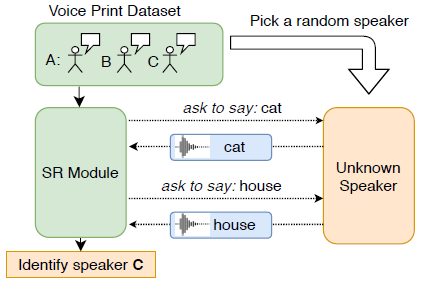
\includegraphics[scale=1.0]{figures/isr_game.png}
    \caption{Схема интерактивной игры по определению диктора \citeisr}
\end{figure}